The inspection of only four bending operations out of six bending are required for the test part. Figure \ref{fig:bending-inspection} shows these inspection camera images upon trigger. Figure \ref{subfig:inspection-1}, \ref{subfig:inspection-5} and \ref{subfig:inspection-6} tests the bending operation of 90\textdegree{} which is performed at bending station 1. Figure \ref{subfig:inspection-2} is the testing of bending of 135\textdegree{} which happens at bending station 2.

Table \ref{tab:bending-data} shows the bending angles as measured by the inspection camera for ten sheet metal parts. The angle measurement is pretty close to each other. The angle is measured by the light reflected by the edge of sheet metal part. Because of different surface roughness and impurities on surface, there is slight deviation in the bending angles measured. A tolerance of 90$\pm5$\textdegree{} is set for the bending 1, bending 5 and bending 6. For bending 2, a tolerance of 135$\pm10$\textdegree{} is set. These tolerance values can be adjusted on the SIMATIC \hyperref[acro:HMI]{HMI}.

\begin{figure}[h]
    \centering
    \begin{subfigure}{0.48\textwidth}
        \centering
        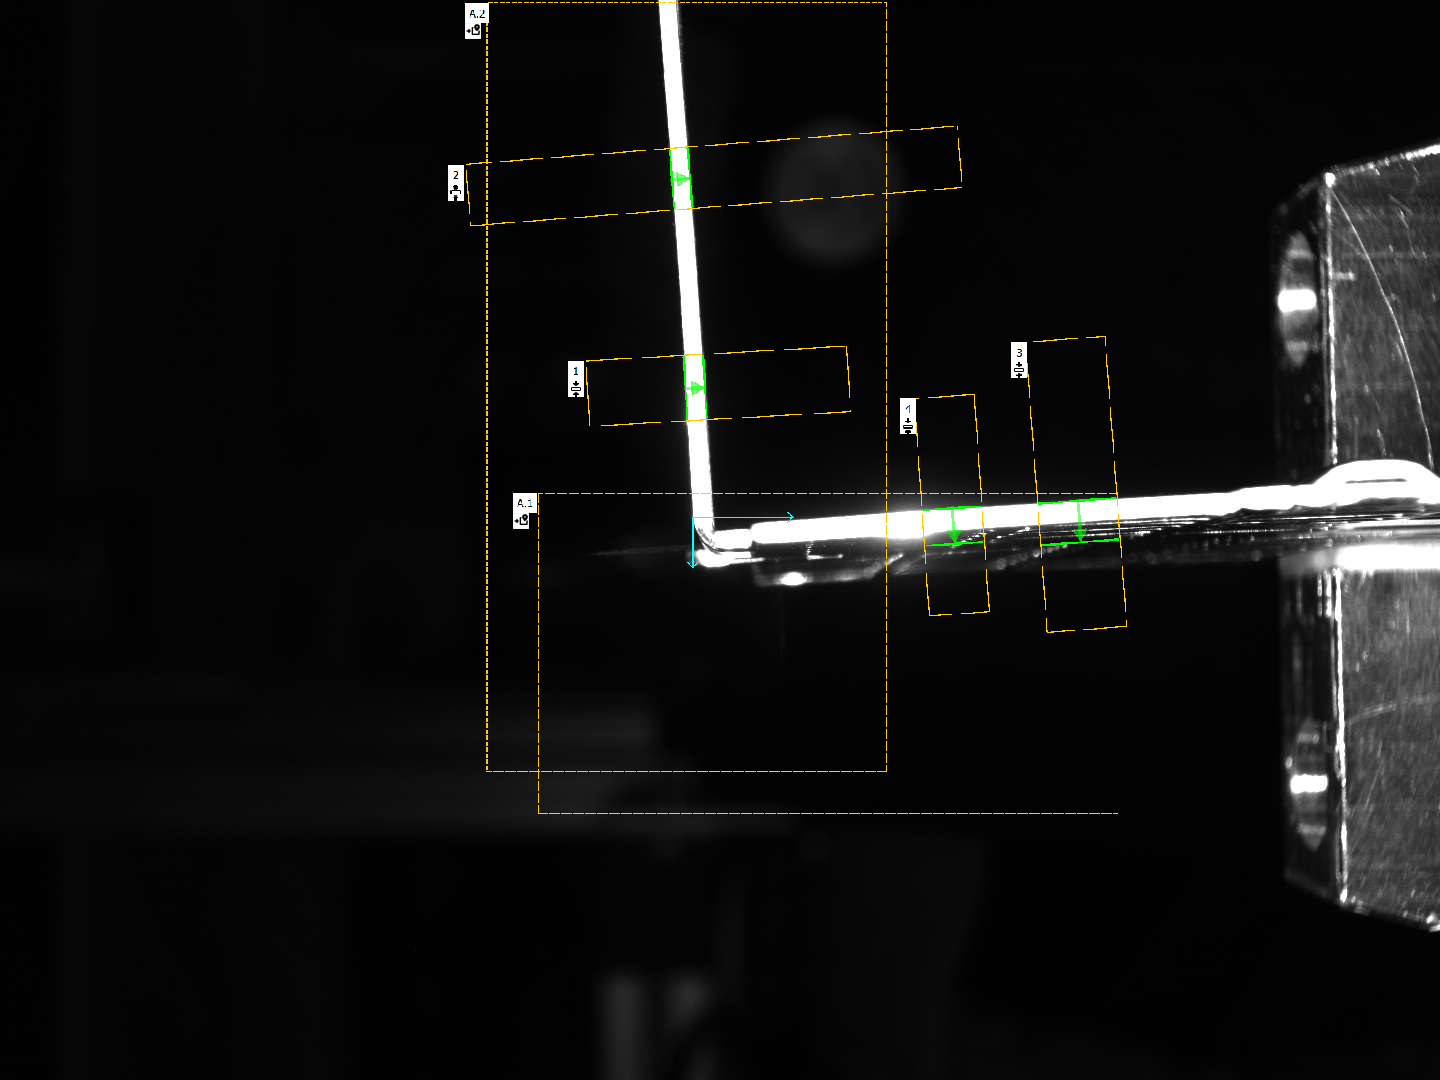
\includegraphics[width=\textwidth]{figures/008_inspection/inpection_1_overlay2.png}
        \caption{bending operation 1}
        \label{subfig:inspection-1}
        \vspace{0.5cm}
    \end{subfigure}\hspace{0.25cm}
    \begin{subfigure}{0.48\textwidth}
        \centering
        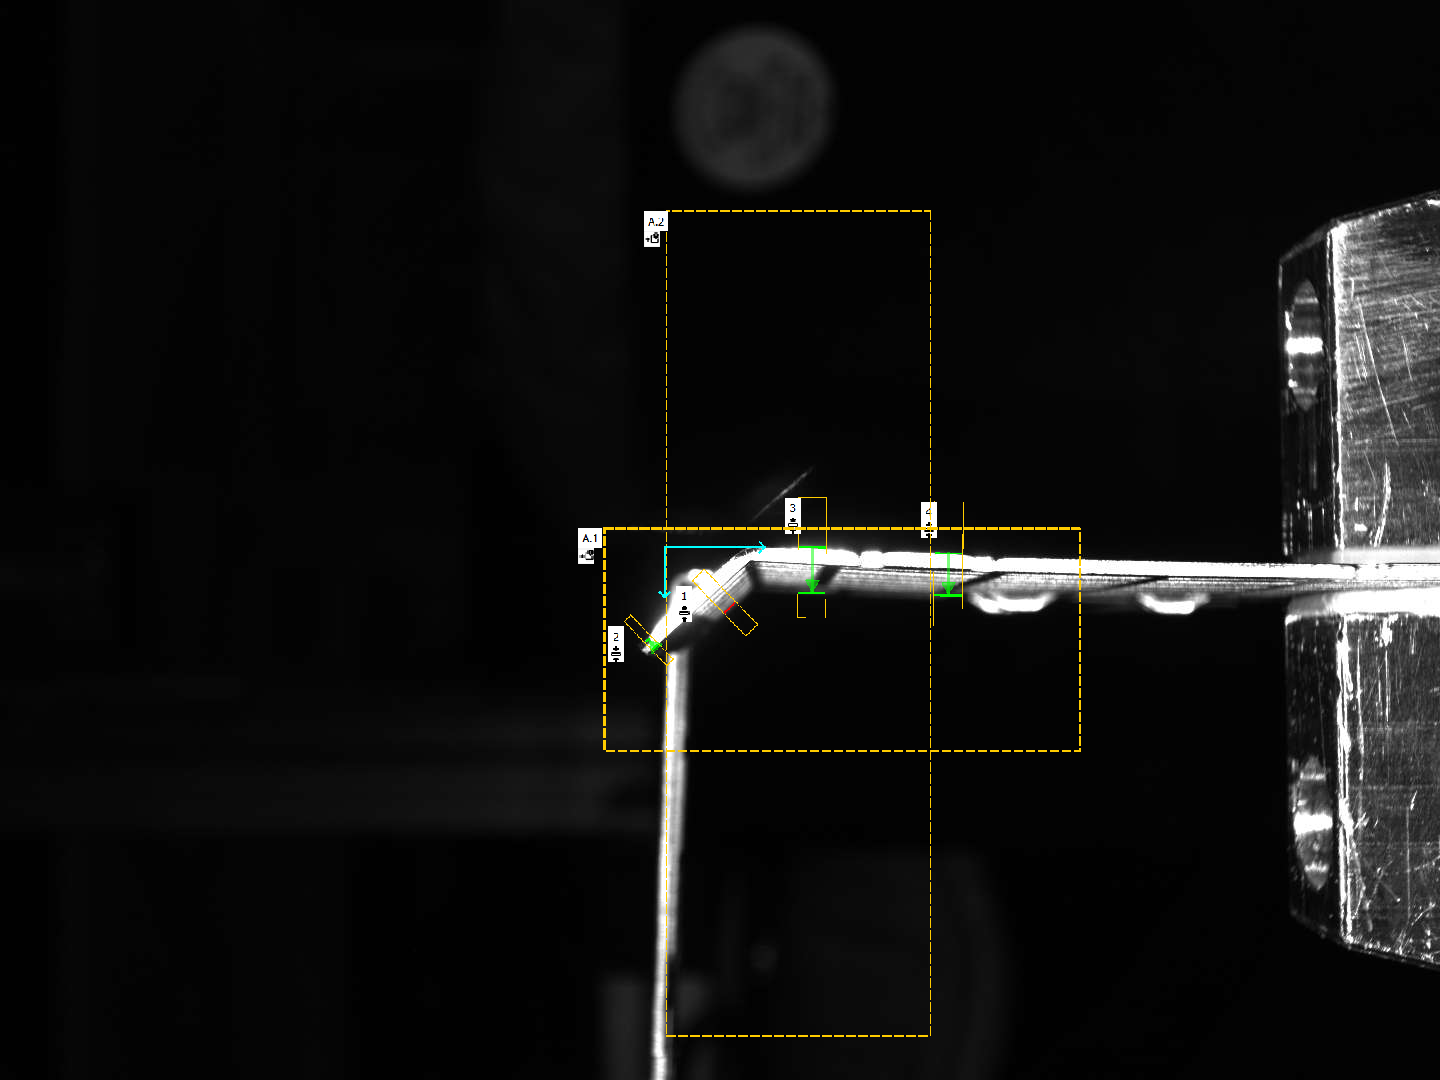
\includegraphics[width=\textwidth]{figures/008_inspection/inspection_2_overlay.png}
        \caption{bending operation 2}
        \label{subfig:inspection-2}
        \vspace{0.5cm}
    \end{subfigure}\hspace{0.25cm}
    \begin{subfigure}{0.48\textwidth}
        \centering
        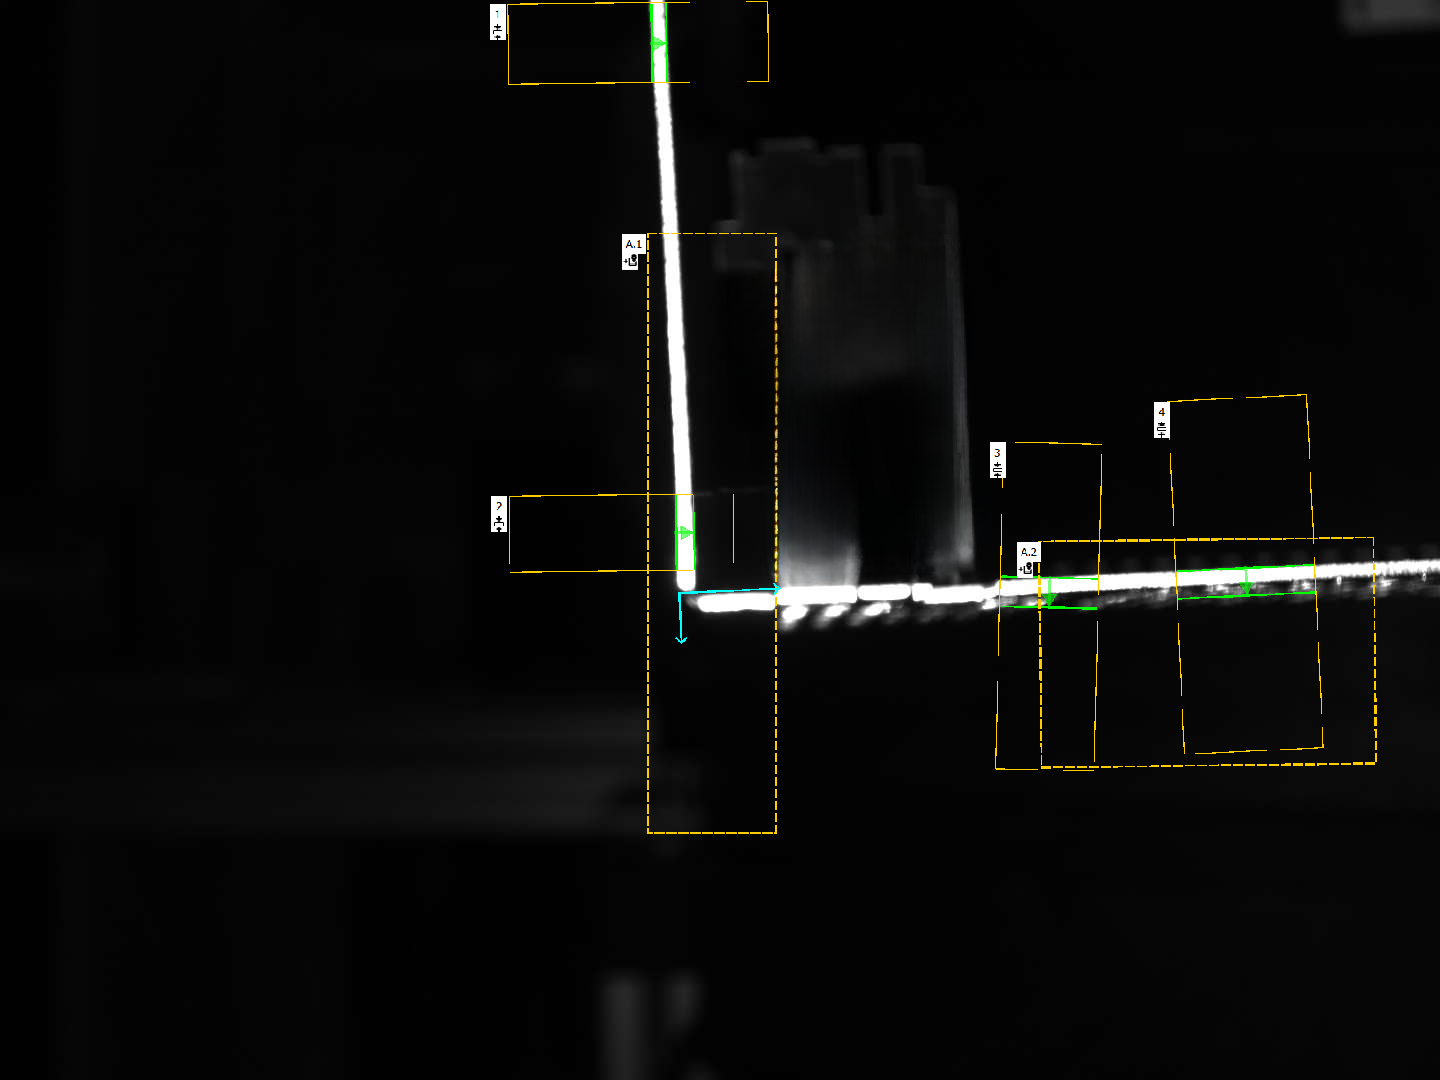
\includegraphics[width=\textwidth]{figures/008_inspection/inspection_5_overlay_cleanup.png}
        \caption{bending operation 5}
        \label{subfig:inspection-5}
        \vspace{0.25cm}
    \end{subfigure}\hspace{0.25cm}
    \begin{subfigure}{0.48\textwidth}
        \centering
        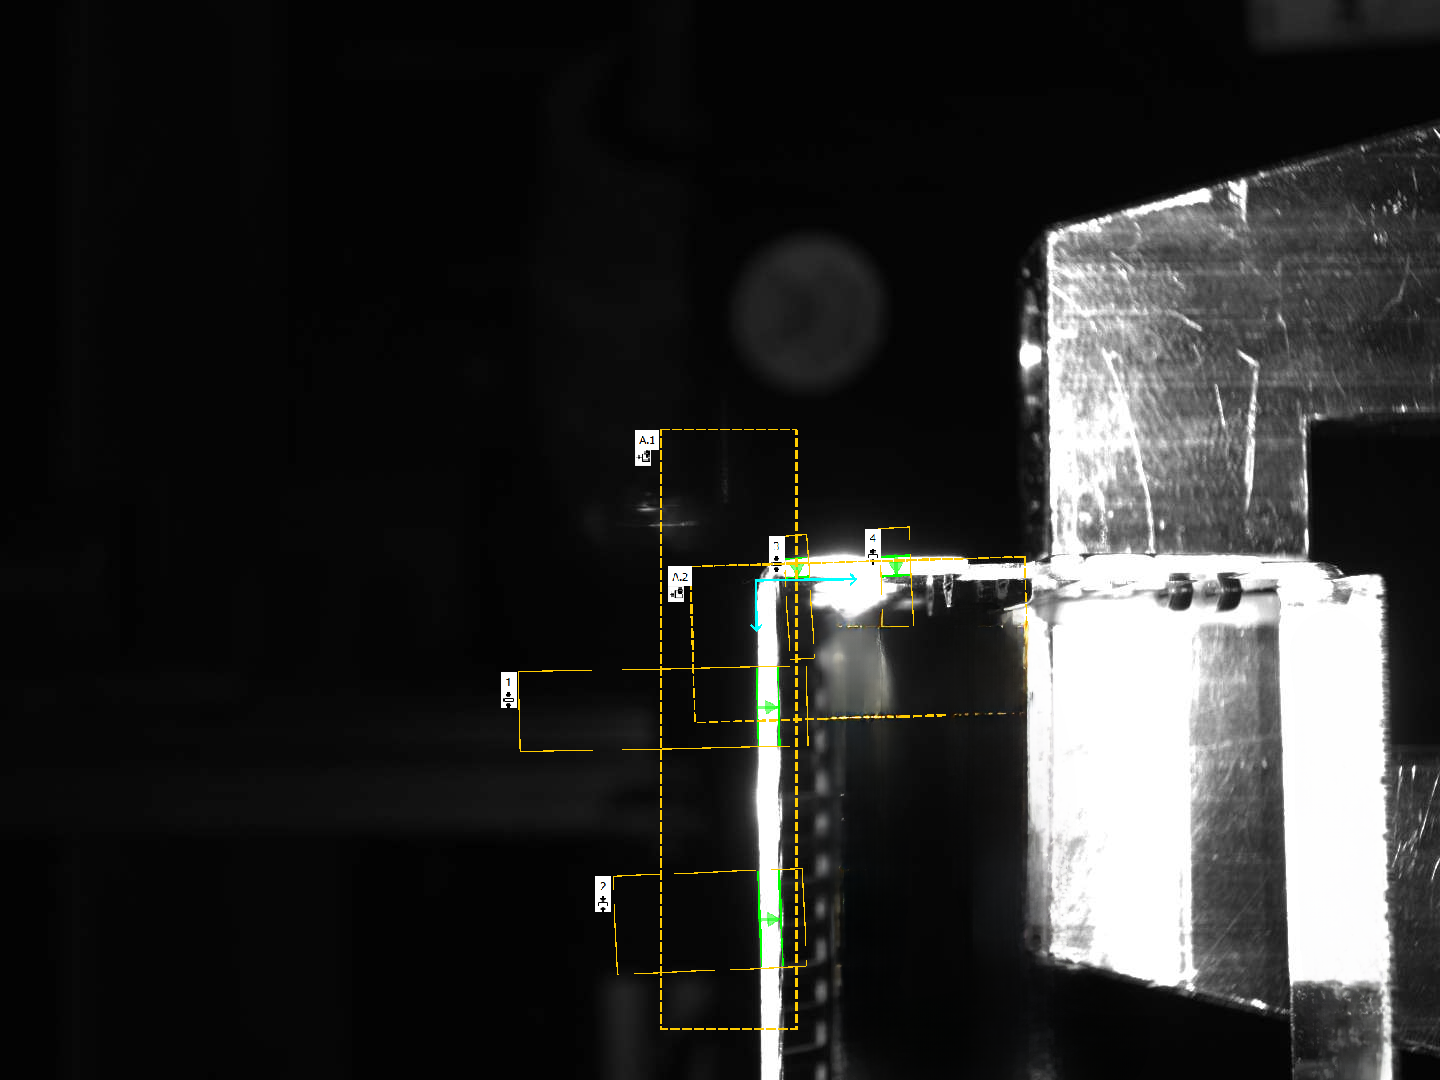
\includegraphics[width=\textwidth]{figures/008_inspection/inspection_6_overlay_cleanup.png}
        \caption{bending operation 6}
        \label{subfig:inspection-6}
        \vspace{0.25cm}
    \end{subfigure}\hspace{0.25cm}
    \caption{Inspection after (a) bending 1 (b) bending 2 (c) bending 5 (d) bending 6}
    \label{fig:bending-inspection}
\end{figure}

\begin{table}[ht]
    \centering
    \small
    \renewcommand{\arraystretch}{1.2} % Adjusts row height
    \begin{tabular}{llcccc}
        & \textbf{Bending 1} & \textbf{Bending 2} & \textbf{Bending 5} & \textbf{Bending 6} \\
        \hline
        & 89.16801 & 133.412 & 88.84901 & 87.79301 \\
        & 89.29201 & 133.048 & 88.77    & 87.36501 \\
        & 89.381   & 133.548 & 88.785   & 87.257   \\
        & 89.344   & 132.454 & 88.928   & 87.561   \\
        & 89.43401 & 133.184 & 89.217   & 87.302   \\
        & 88.402   & 132.967 & 89.176   & 88.19701 \\
        & 89.10001 & 134.015 & 88.926   & 88.276   \\
        & 90.08801 & 132.146 & 89.023   & 87.58801 \\
        & 90.08701 & 134.084 & 87.966   & 87.75301 \\
        & 89.995   & 135.314 & 88.34801 & 87.526   \\
        \hline
    \end{tabular}
    \caption{Bending angle as measured by inspection camera}
    \label{tab:bending-data}
\end{table}

The bending angles measured by the inspection camera are saved by the \hyperref[acro:PLC]{PLC} in a \textit{.csv} file. SIMATIC \hyperref[acro:HMI]{HMI} also shows the current cycle bending angles for the operator to overview the current status of bending operation. This \textit{.csv} file provides insights in the quality of bending process. It is evident from the angles captured that the bending process is consistent over time, without any requirement for a new calibration.